\documentclass[ignorenonframetext,12pt,t]{beamer}
\setbeamertemplate{caption}[numbered]
\setbeamertemplate{caption label separator}{: }
\setbeamercolor{caption name}{fg=normal text.fg}
\beamertemplatenavigationsymbolsempty
\usepackage{lmodern}
\usepackage{amssymb,amsmath}
\usepackage{ifxetex,ifluatex}
\usepackage{fixltx2e} % provides \textsubscript
\ifnum 0\ifxetex 1\fi\ifluatex 1\fi=0 % if pdftex
  \usepackage[T1]{fontenc}
  \usepackage[utf8]{inputenc}
\else % if luatex or xelatex
  \ifxetex
    \usepackage{mathspec}
  \else
    \usepackage{fontspec}
  \fi
  \defaultfontfeatures{Ligatures=TeX,Scale=MatchLowercase}
\fi
\usetheme{Honefoss}
% use upquote if available, for straight quotes in verbatim environments
\IfFileExists{upquote.sty}{\usepackage{upquote}}{}
% use microtype if available
\IfFileExists{microtype.sty}{%
\usepackage{microtype}
\UseMicrotypeSet[protrusion]{basicmath} % disable protrusion for tt fonts
}{}
\newif\ifbibliography
\usepackage{graphicx,grffile}
\makeatletter
\def\maxwidth{\ifdim\Gin@nat@width>\linewidth\linewidth\else\Gin@nat@width\fi}
\def\maxheight{\ifdim\Gin@nat@height>\textheight0.8\textheight\else\Gin@nat@height\fi}
\makeatother
% Scale images if necessary, so that they will not overflow the page
% margins by default, and it is still possible to overwrite the defaults
% using explicit options in \includegraphics[width, height, ...]{}
\setkeys{Gin}{width=\maxwidth,height=\maxheight,keepaspectratio}

% Prevent slide breaks in the middle of a paragraph:
\widowpenalties 1 10000
\raggedbottom

\AtBeginPart{
  \let\insertpartnumber\relax
  \let\partname\relax
  \frame{\partpage}
}
\AtBeginSection{
  \ifbibliography
  \else
    \let\insertsectionnumber\relax
    \let\sectionname\relax
    \frame{\sectionpage}
  \fi
}
\AtBeginSubsection{
  \let\insertsubsectionnumber\relax
  \let\subsectionname\relax
  \frame{\subsectionpage}
}

\setlength{\emergencystretch}{3em}  % prevent overfull lines
\providecommand{\tightlist}{%
  \setlength{\itemsep}{0pt}\setlength{\parskip}{0pt}}
\setcounter{secnumdepth}{0}

\title{Where}
\subtitle{A new geodetic software being developed at the Norwegian Mapping
Authority}
\author{Geir Arne Hjelle}
\date{May 26, 2016}

\begin{document}
\frame{\titlepage}

\begin{frame}{A short history}

The \textbf{Where} project was started in the fall of 2015 with the goal
of building software that can analyse and combine data for \emph{VLBI},
\emph{SLR}, \emph{GNSS} and \emph{DORIS}.

\begin{itemize}
\item
  \textbf{Where} builds on ideas and experiences from the \emph{Geosat}
  software
\item
  The \textbf{Where-team} consists of five researchers at the Norwegian
  Mapping Authority (NMA):

  \begin{itemize}
  \tightlist
  \item
    Michael Dähnn (GPS)
  \item
    Ingrid Fausk (SLR)
  \item
    Geir Arne Hjelle (VLBI, GPS)
  \item
    Ann-Silje Kirkvik (VLBI)
  \item
    Eirik Mysen (VLBI)
  \end{itemize}
\item
  NMA is currently building / expanding the observatory at Ny-Ålesund
\end{itemize}

\end{frame}

\begin{frame}{The new Ny-Ålesund observatory}

\begin{figure}[htbp]
\centering
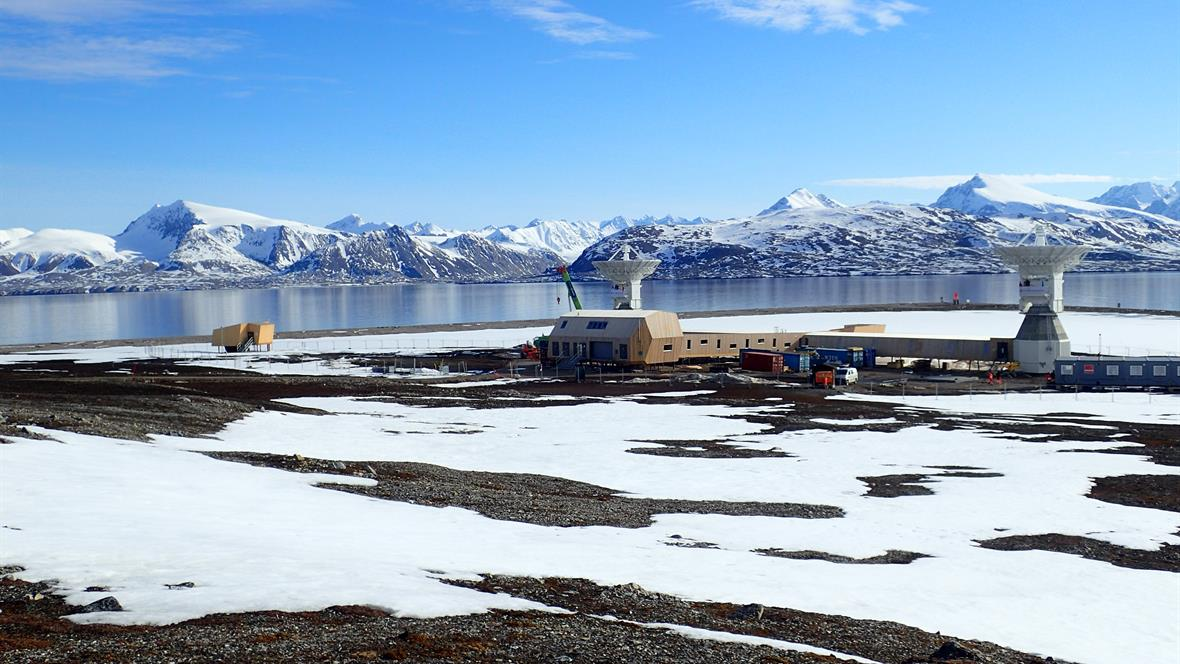
\includegraphics{nyal_antennas.jpg}
\caption{VLBI antennas were installed last week}
\end{figure}

\end{frame}

\begin{frame}{Current status}

\begin{itemize}
\item
  All models from the \emph{IERS Conventions} are implemented for
  \emph{VLBI} and \emph{SLR}

  \begin{itemize}
  \item
    Many of the models can be reused for the other techniques
  \item
    We participated in a \emph{VLBI Analysis Software Comparison
    Campaign} organized by Onsala with \emph{Geosat}, and are currently
    testing \textbf{Where} against these results
  \item
    We are almost done with an orbit integrator for \emph{SLR}
    satellites
  \end{itemize}
\item
  We are currently working on Precise Point Positioning (PPP) for
  \emph{GPS}
\item
  We have only done very simple tests for \emph{DORIS} data so far
\end{itemize}

\end{frame}

\begin{frame}[fragile]{Technology}

The \textbf{Where} software is mainly being written in \emph{Python}

\begin{itemize}
\item
  Solid, flexible and fast libraries like \texttt{numpy},
  \texttt{astropy}, \texttt{matplotlib} and \texttt{scipy} are available
\item
  We use a \textbf{HDF5}-based format for storing data while the program
  is running
\item
  \emph{Python} has effective interfaces to \emph{C} and \emph{Fortran}
  code, and we can use the \textbf{Sofa} and \textbf{IERS} software
  libraries directly
\end{itemize}

\end{frame}

\begin{frame}{Technology -- plans}

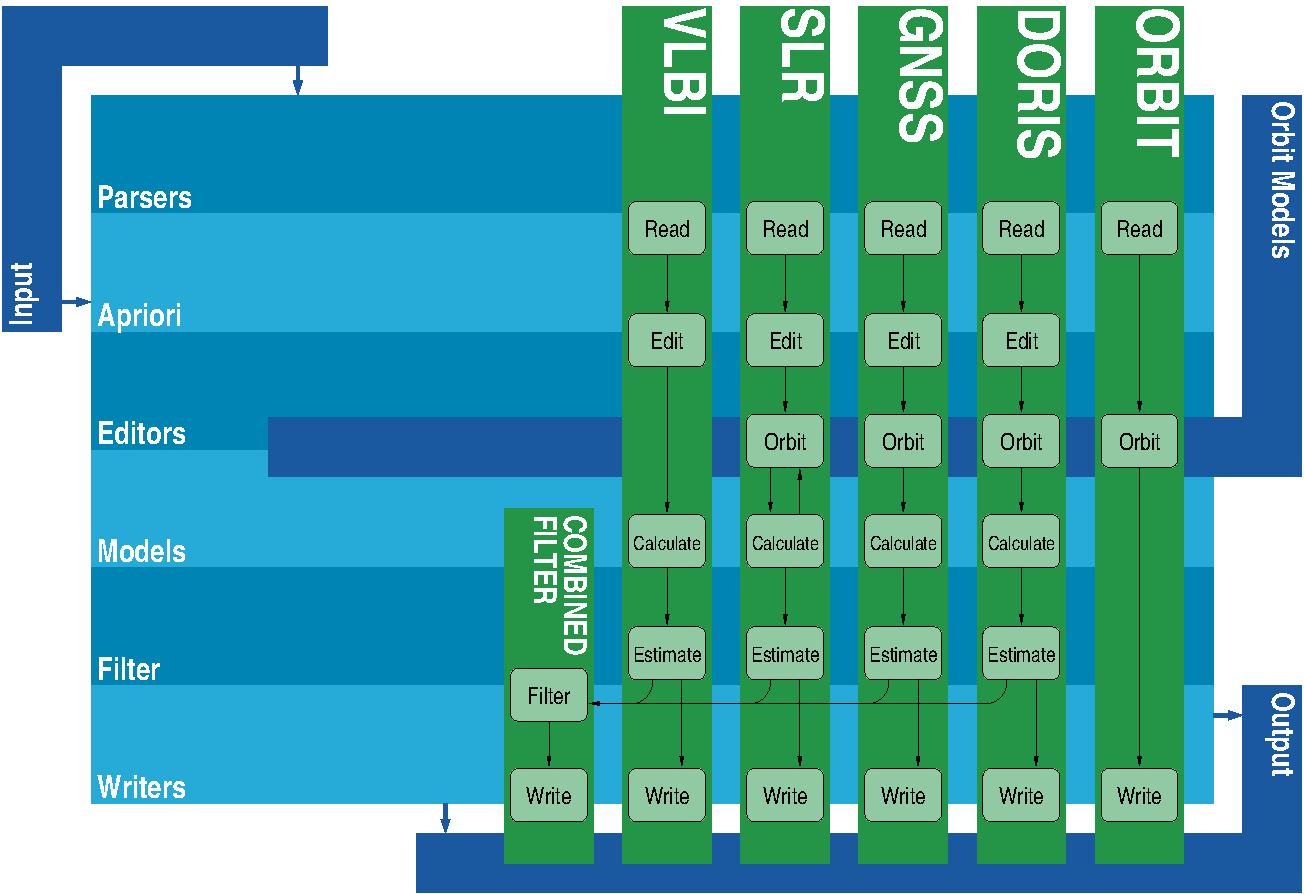
\includegraphics{../../../monitor/figure/code_structure}

\end{frame}

\begin{frame}{Technology -- current}

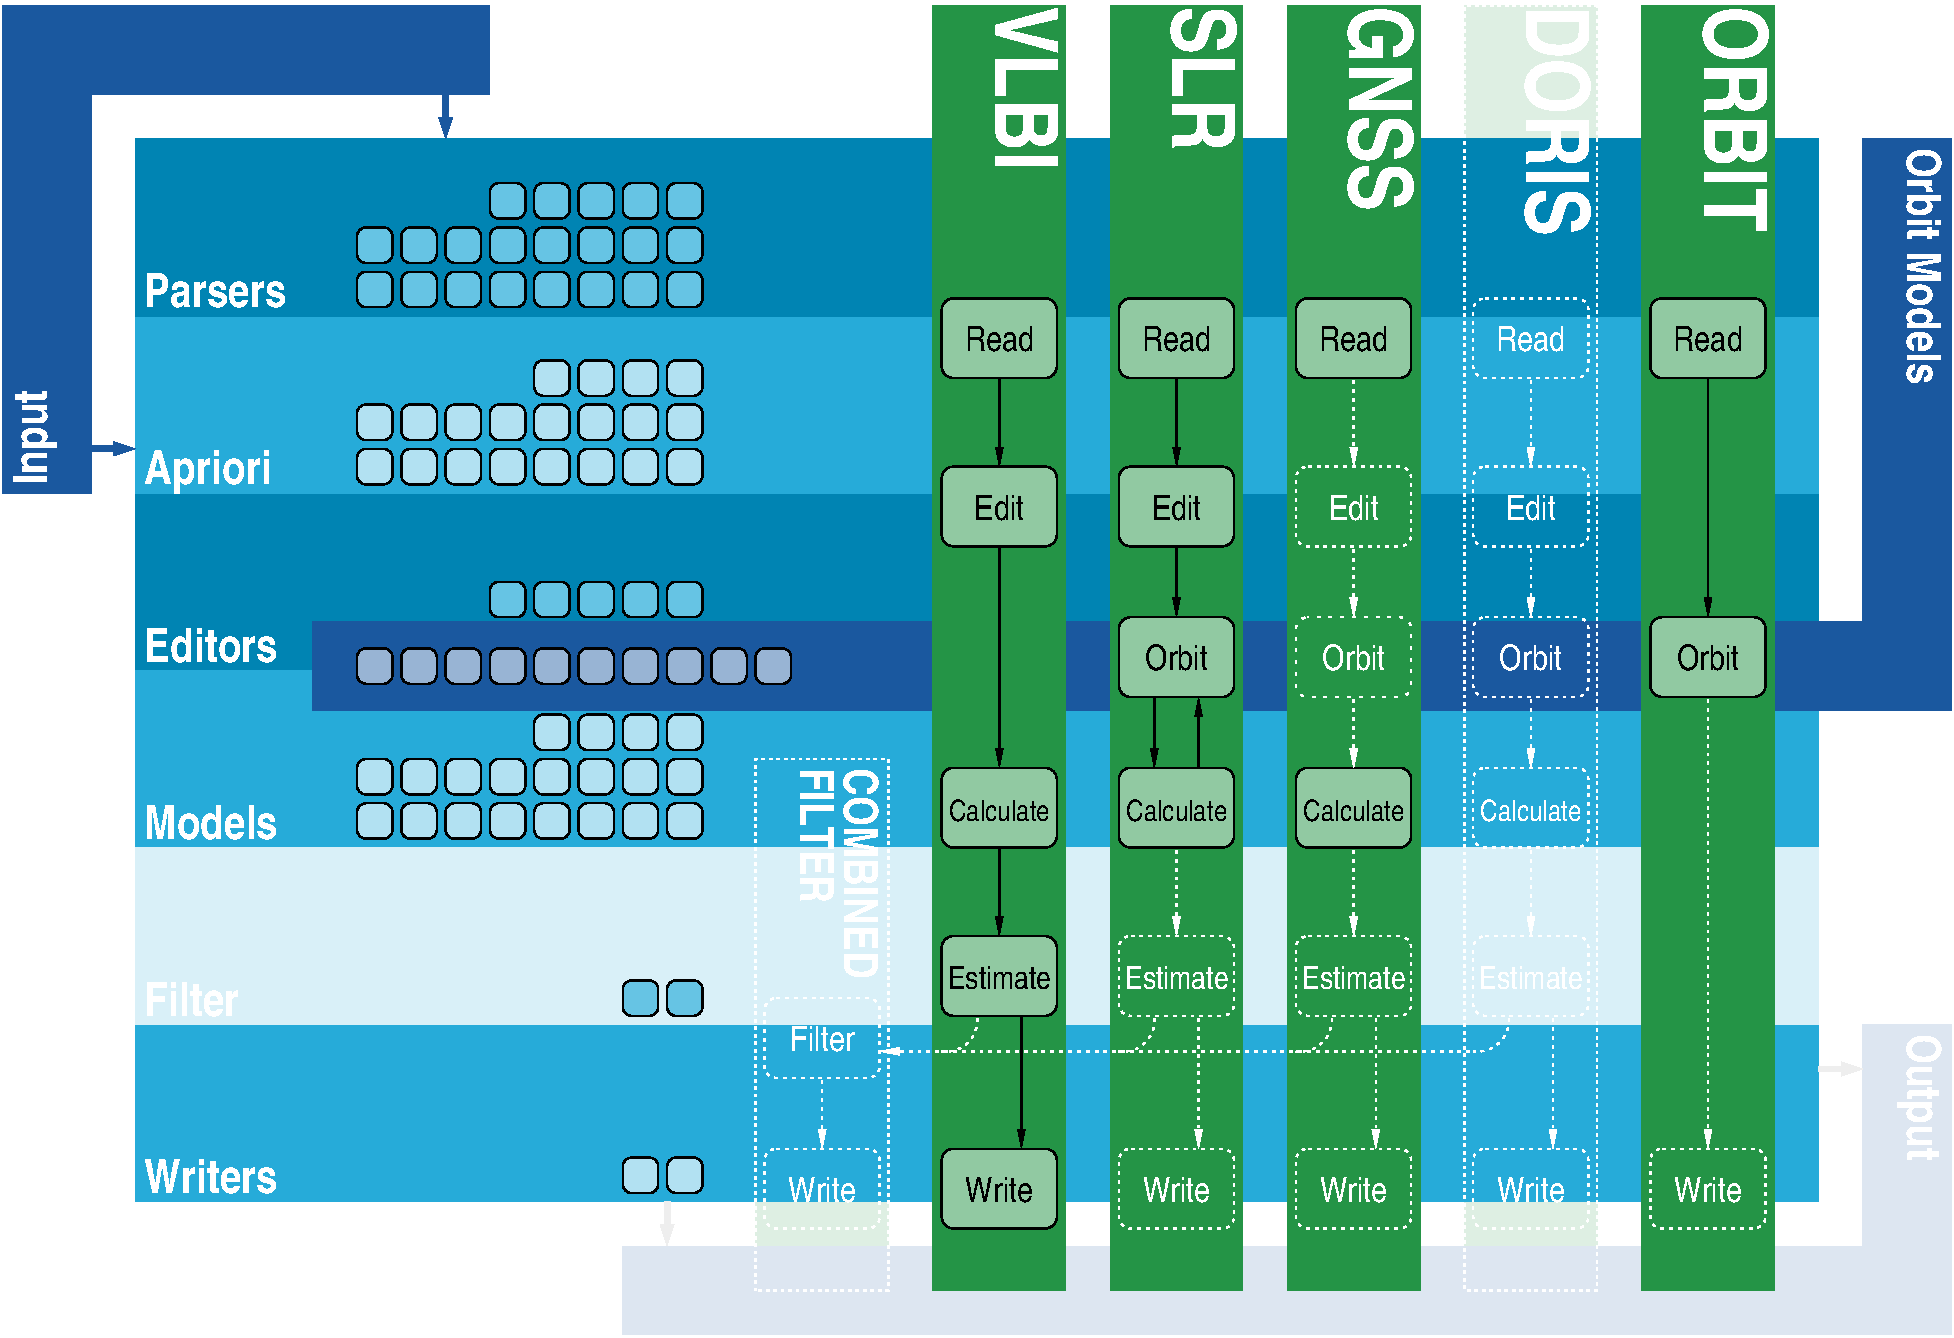
\includegraphics{../../../monitor/figure/code_structure_current}

\end{frame}

\begin{frame}{Future plans}

At the moment, the highest priorities for \textbf{Where} are

\begin{itemize}
\item
  finishing the \emph{VLBI} analysis

  \begin{itemize}
  \item
    The filter / estimation module
  \item
    Proper output and reporting
  \end{itemize}
\item
  finishing the \emph{SLR} analysis

  \begin{itemize}
  \tightlist
  \item
    The orbit integrator needs some more work
  \end{itemize}
\item
  finishing PPP for \emph{GPS} and starting to look at \emph{Galileo}
  and possibly \emph{Glonass}

  \begin{itemize}
  \tightlist
  \item
    Orbit integration for GNSS-satellites
  \end{itemize}
\end{itemize}

\end{frame}

\begin{frame}{Where is \emph{DORIS}?}

Unfortunately \emph{DORIS} has been put somewhat on hold due to lack of
resources. However,

\begin{itemize}
\item
  we implemented a \emph{DORIS}-Rinex 3-parser in an early prototype of
  the software
\item
  we did some experimental analysis in the old \emph{Geosat} software
\item
  we hope to do some simple tests quite soon

  \begin{itemize}
  \tightlist
  \item
    use Rinex 3-data and given orbits
  \end{itemize}
\item
  the proper implementation of \emph{DORIS} will be after \emph{VLBI} is
  finished

  \begin{itemize}
  \tightlist
  \item
    many models can be reused from the other techniques
  \end{itemize}
\end{itemize}

\end{frame}

\end{document}
